\documentclass[12pt,a4paper]{article}
\usepackage{preamble}

%%%%%%%%%%%%%%%%%%%%%%%%%%%%%%%%%%%%%%%%%%
%%%% Edit These for yourself
%%%%%%%%%%%%%%%%%%%%%%%%%%%%%%%%%%%%%%%%%%
\newcommand\course{ASC1}
\newcommand\hwnumber{1}
\newcommand\userID{S1910595010, Paul Hörmann}

\begin{document}

\section*{Aufgabe 1: Polynome}
\begin{enumerate}[leftmargin=!,labelindent=5pt]
	\item \textit{\textbf{Simple}} implementation:
		\lstinputlisting[caption={Polynom Common}]{../../matlab/pcommon.m}
		\newpage

	\item \textit{\textbf{Smart}} implementation:
		\lstinputlisting[caption={Polynom Advanced}]{../../matlab/padvanced.m}
		\newpage

	\item Run 1
		\begin{figure}[H]
			\centering
			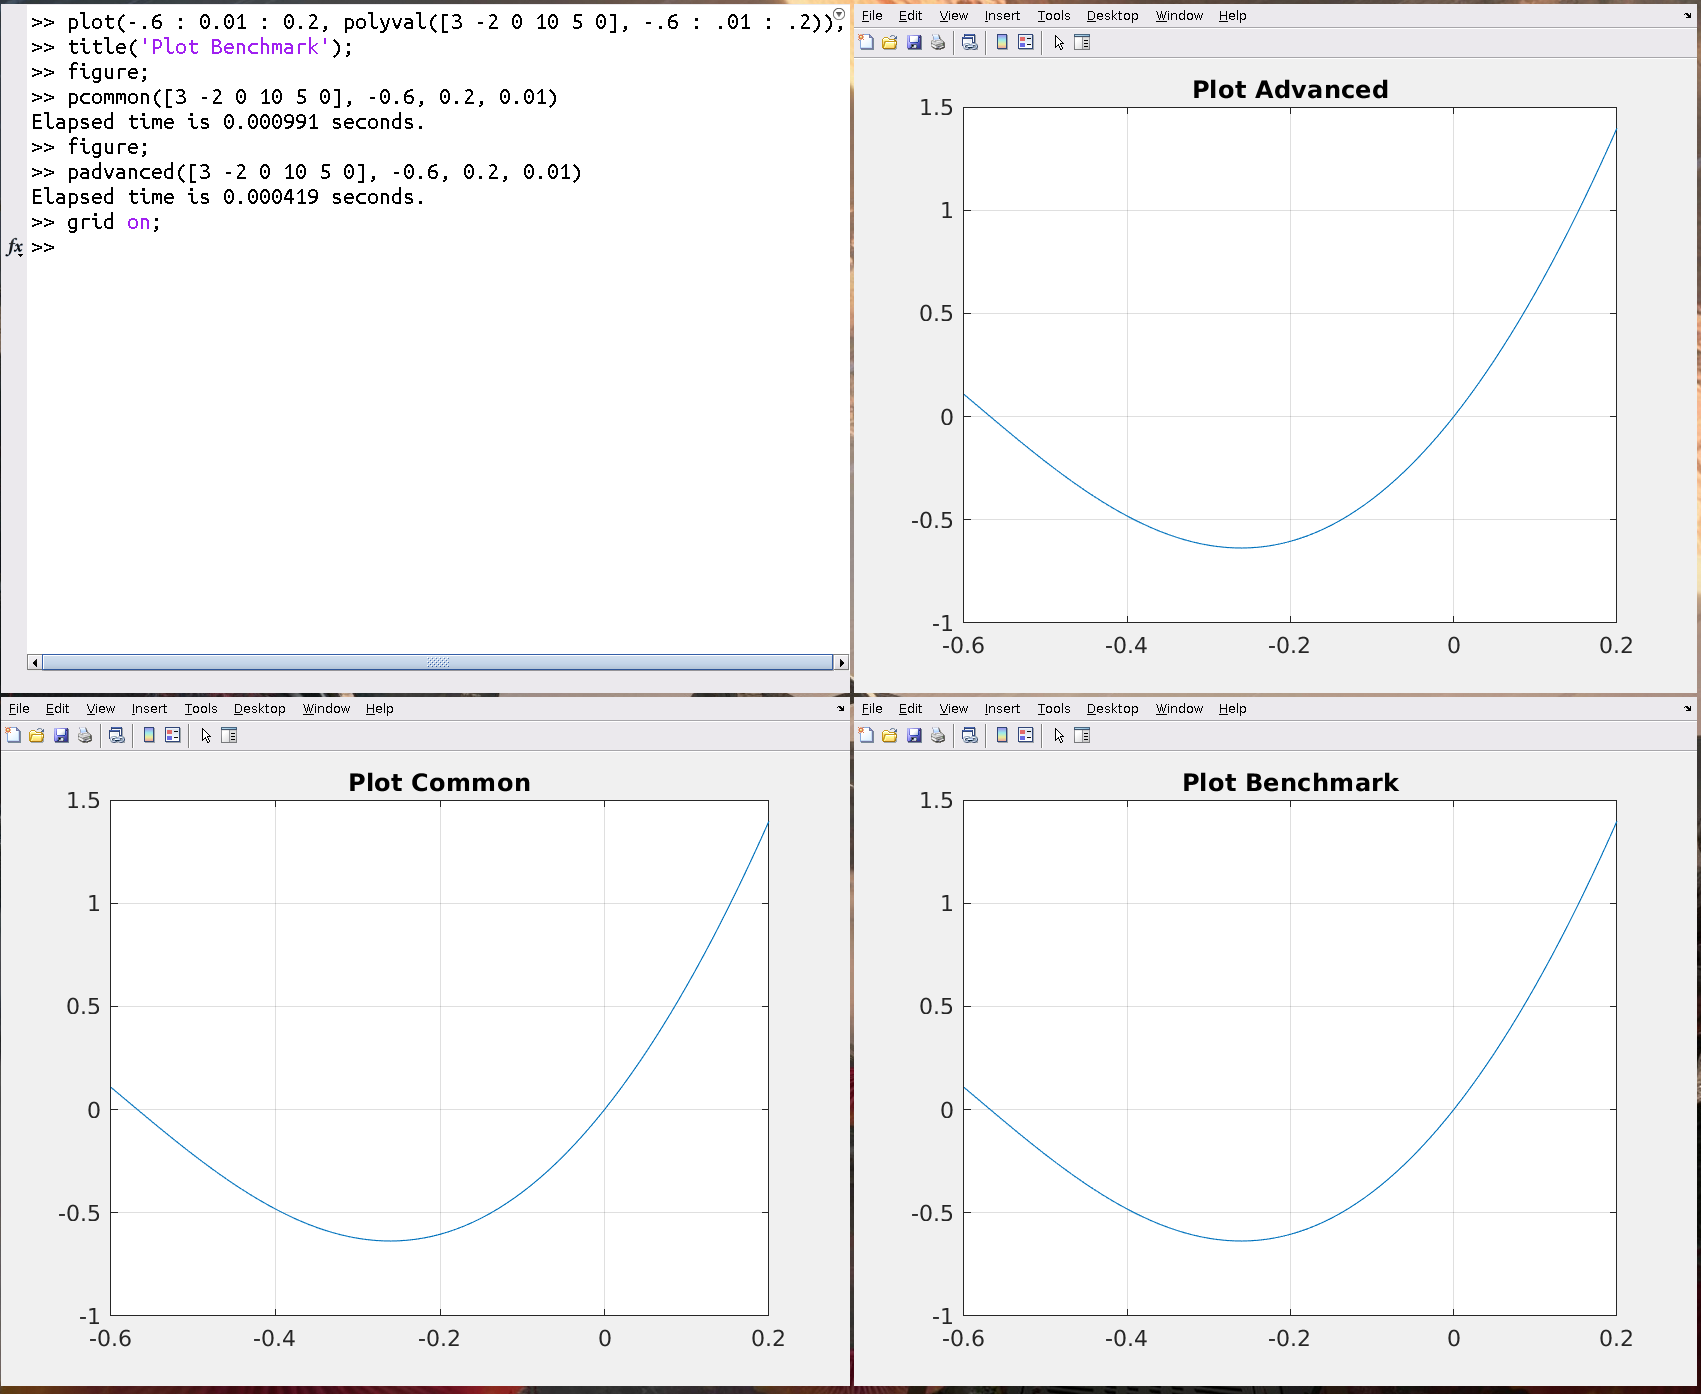
\includegraphics[scale=0.45]{./img/poly_comp_01.png}
		\end{figure}

	\item Run 2
		\begin{figure}[H]
			\centering
			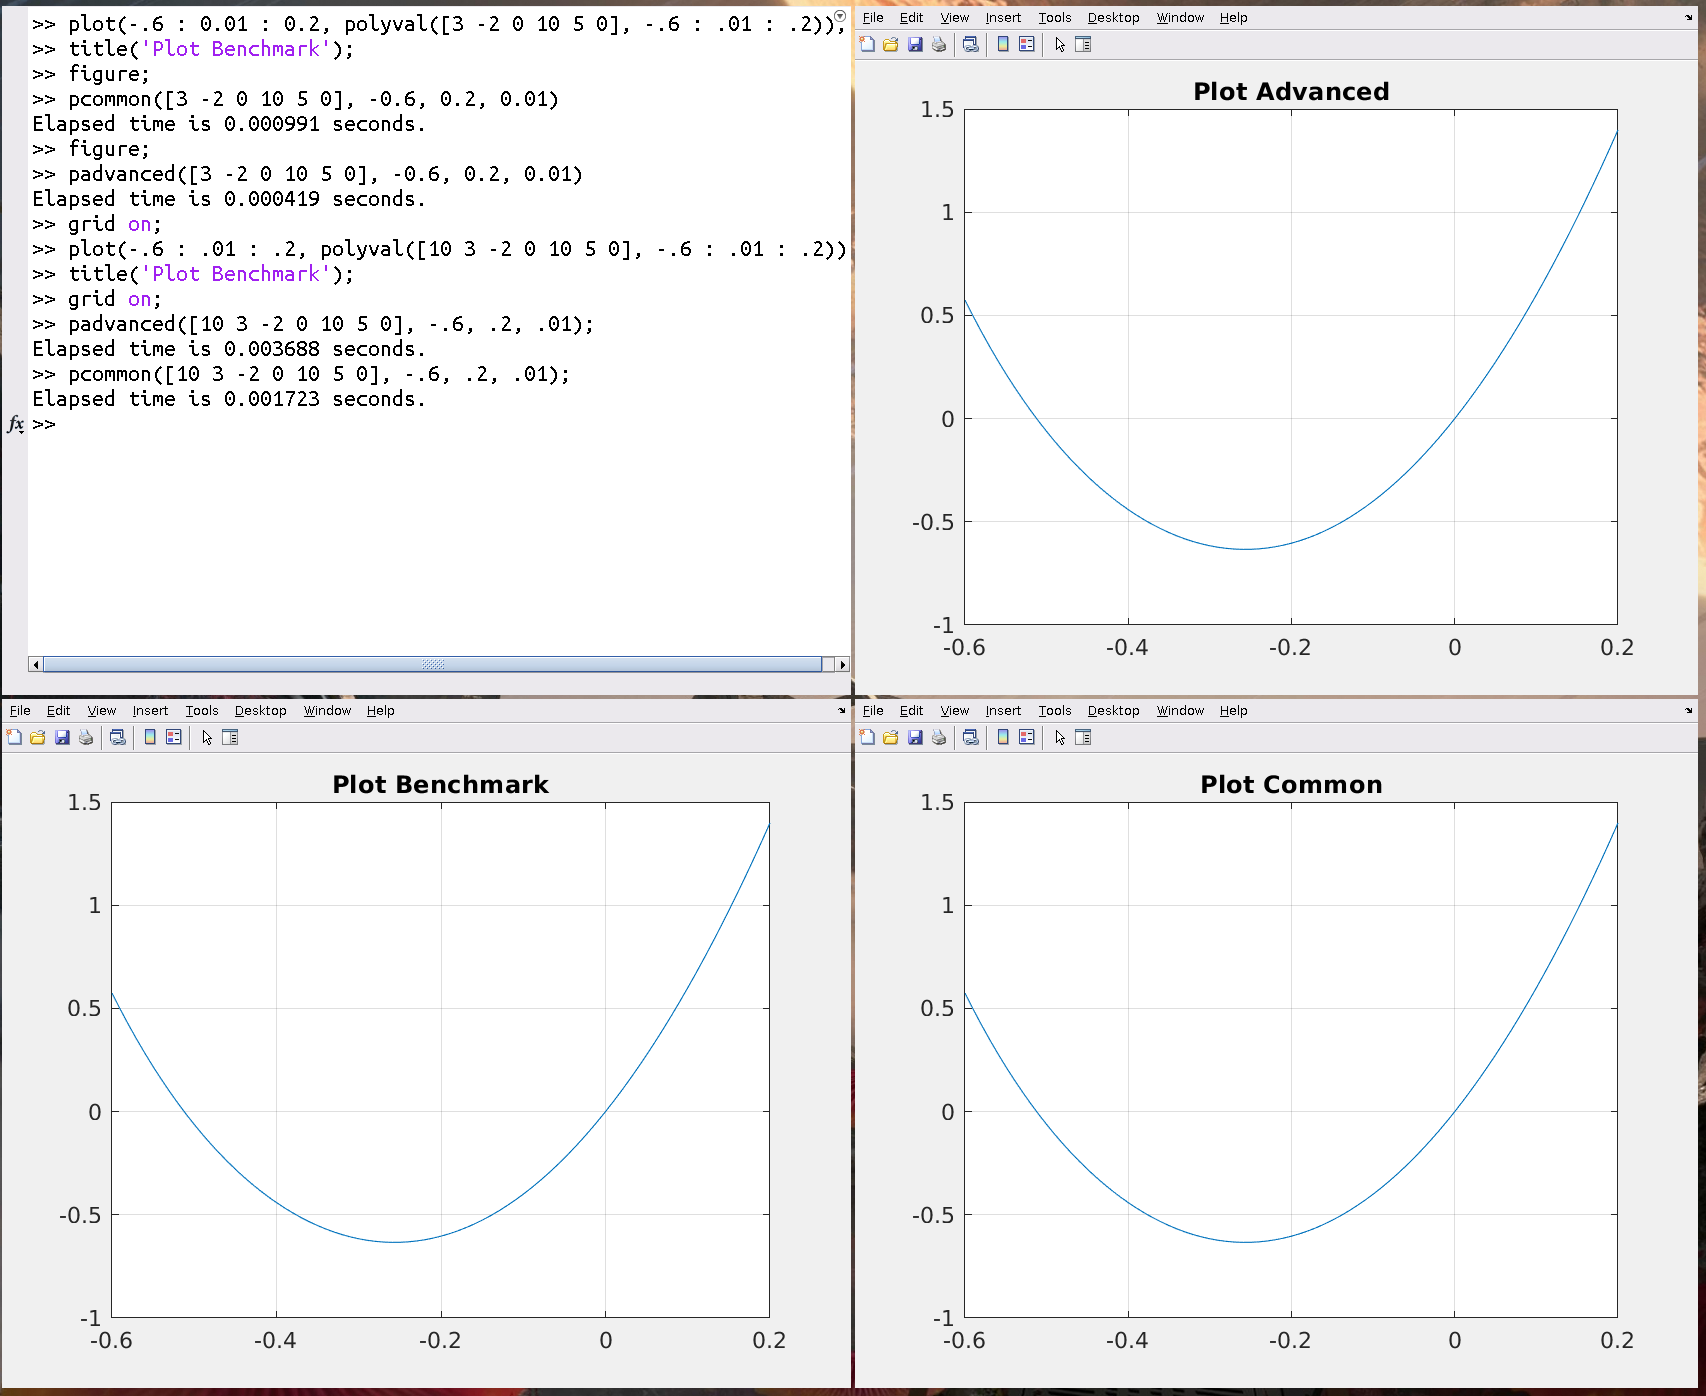
\includegraphics[scale=0.45]{./img/poly_comp_02.png}
		\end{figure}
		\newpage

	\item Run 3
		\begin{figure}[H]
			\centering
			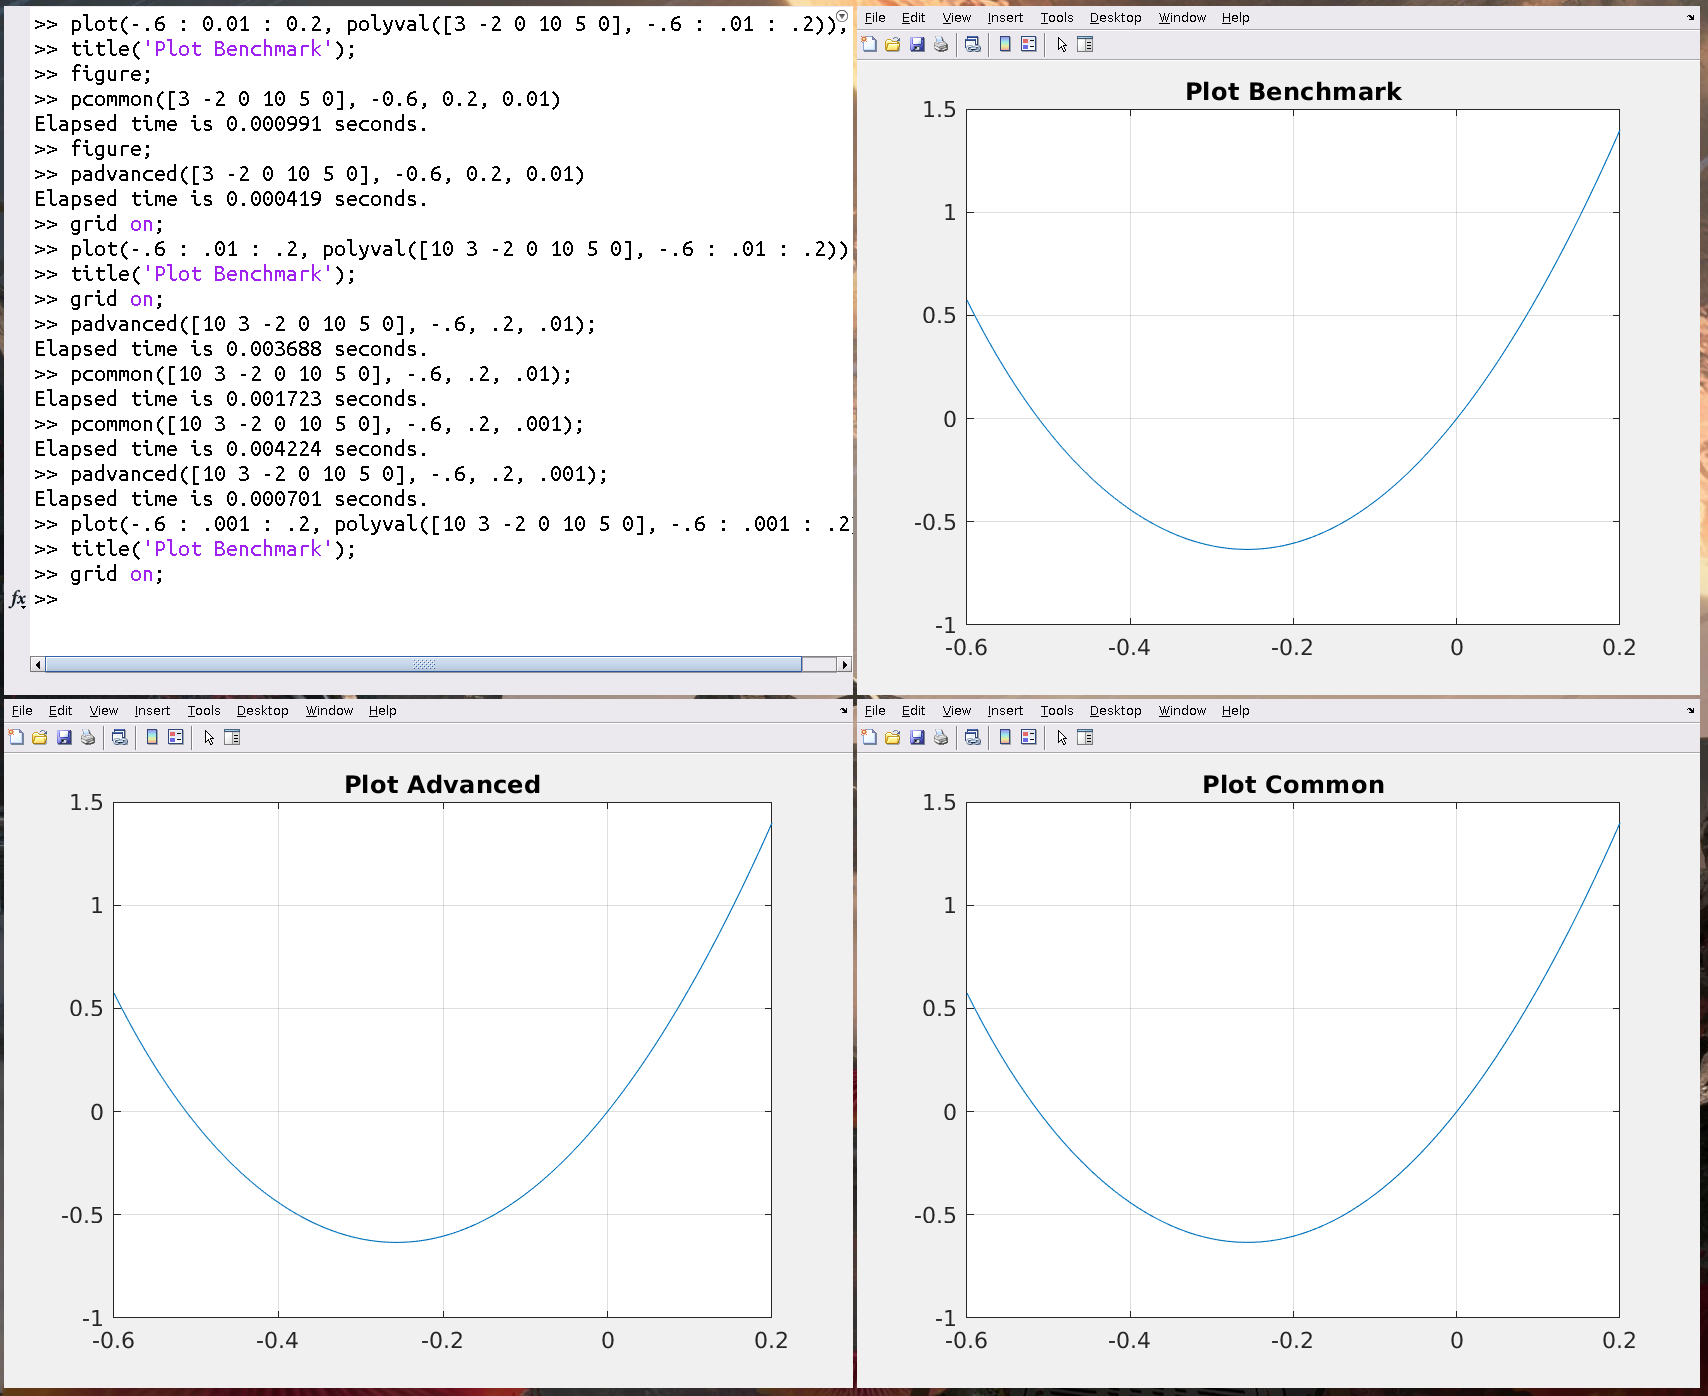
\includegraphics[scale=0.45]{./img/poly_comp_03.png}
		\end{figure}

	\item \textbf{Comparison:}
		\newline
		\newline The advanced implementation is about 5 times faster than the simple one
		in the above three runs.
\end{enumerate}
\newpage

\section*{Aufgabe 2: Malen nach Zahlen (Pt 1)}
\begin{enumerate}[leftmargin=!,labelindent=5pt]
	\item Source Code:
		\lstinputlisting[caption={paint.m}]{../../matlab/paint.m}
		\newpage

	\item Run 1
		\begin{figure}[H]
			\centering
			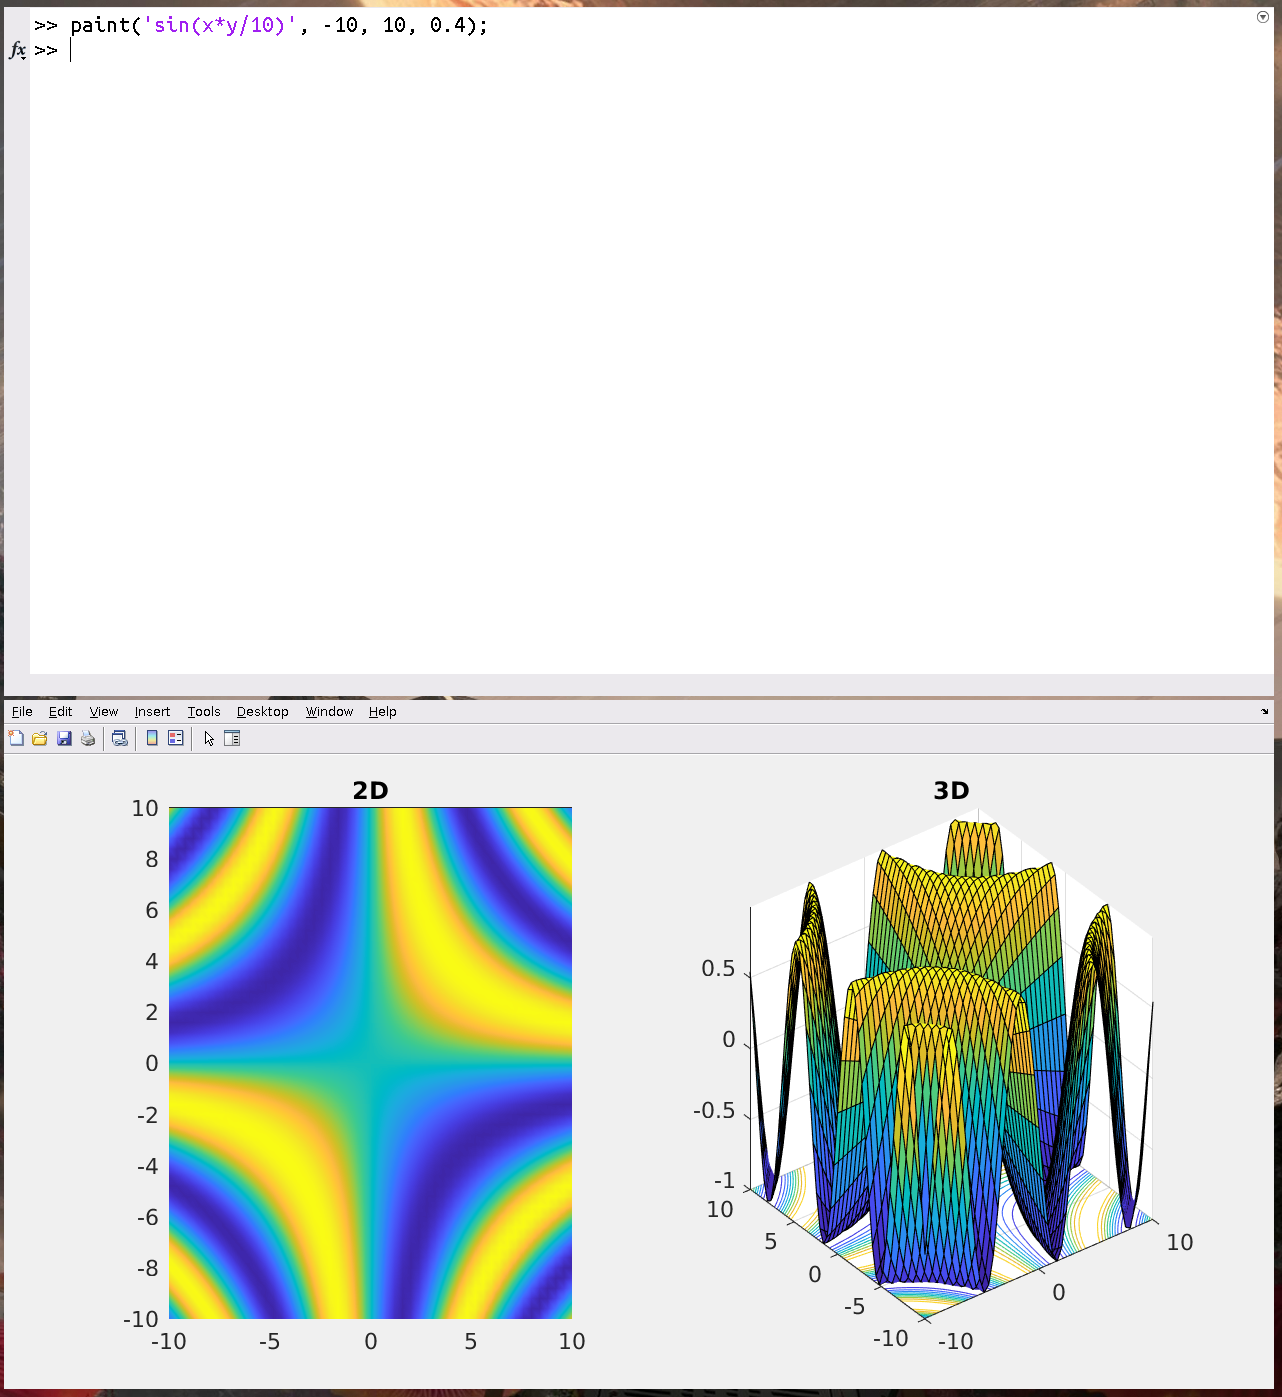
\includegraphics[scale=0.7]{./img/paint_01.png}
		\end{figure}
		\newpage

	\item Run 2
		\begin{figure}[H]
			\centering
			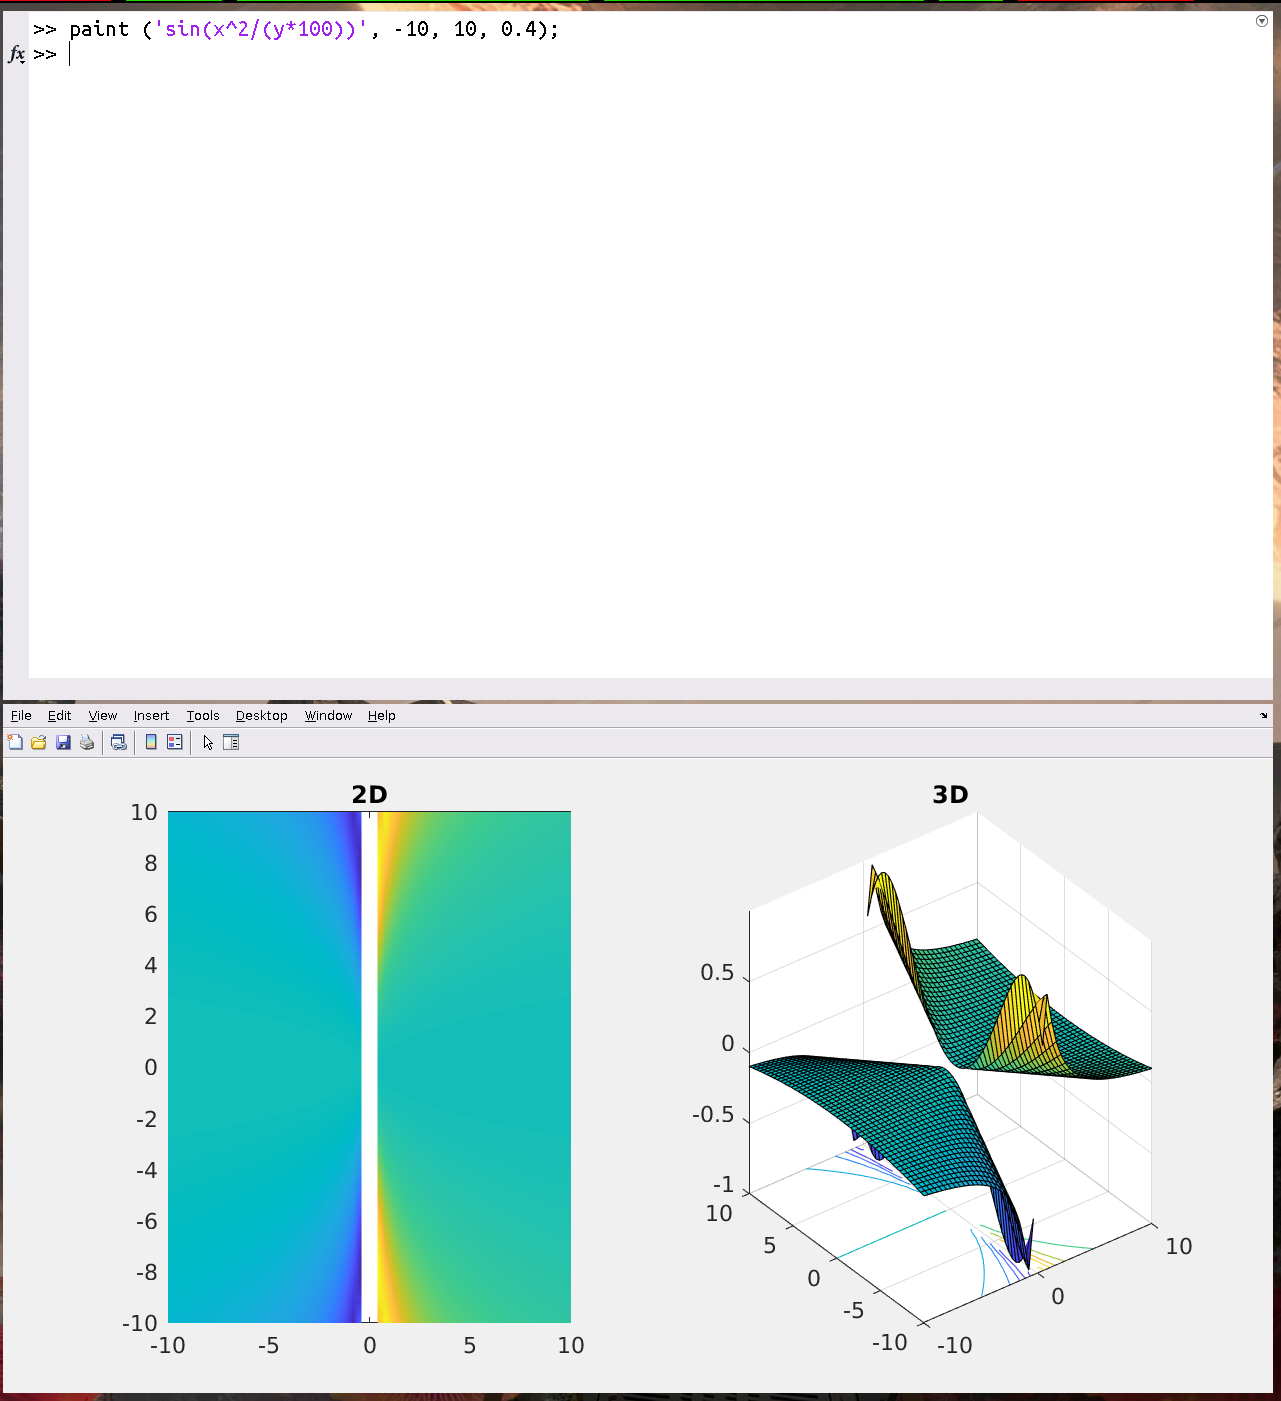
\includegraphics[scale=0.7]{./img/paint_02.png}
		\end{figure}
\end{enumerate}
\newpage

\section*{Aufgabe 3: Malen nach Zahlen (Pt 2)}
\begin{enumerate}[leftmargin=!,labelindent=5pt]
	\item Source Code:
		\lstinputlisting[caption={multidist.m}]{../../matlab/multidist.m}
		\lstinputlisting[caption={multidistPainter.m}]{../../matlab/multidistPainter.m}

	\item Run 1
		\begin{figure}[H]
			\centering
			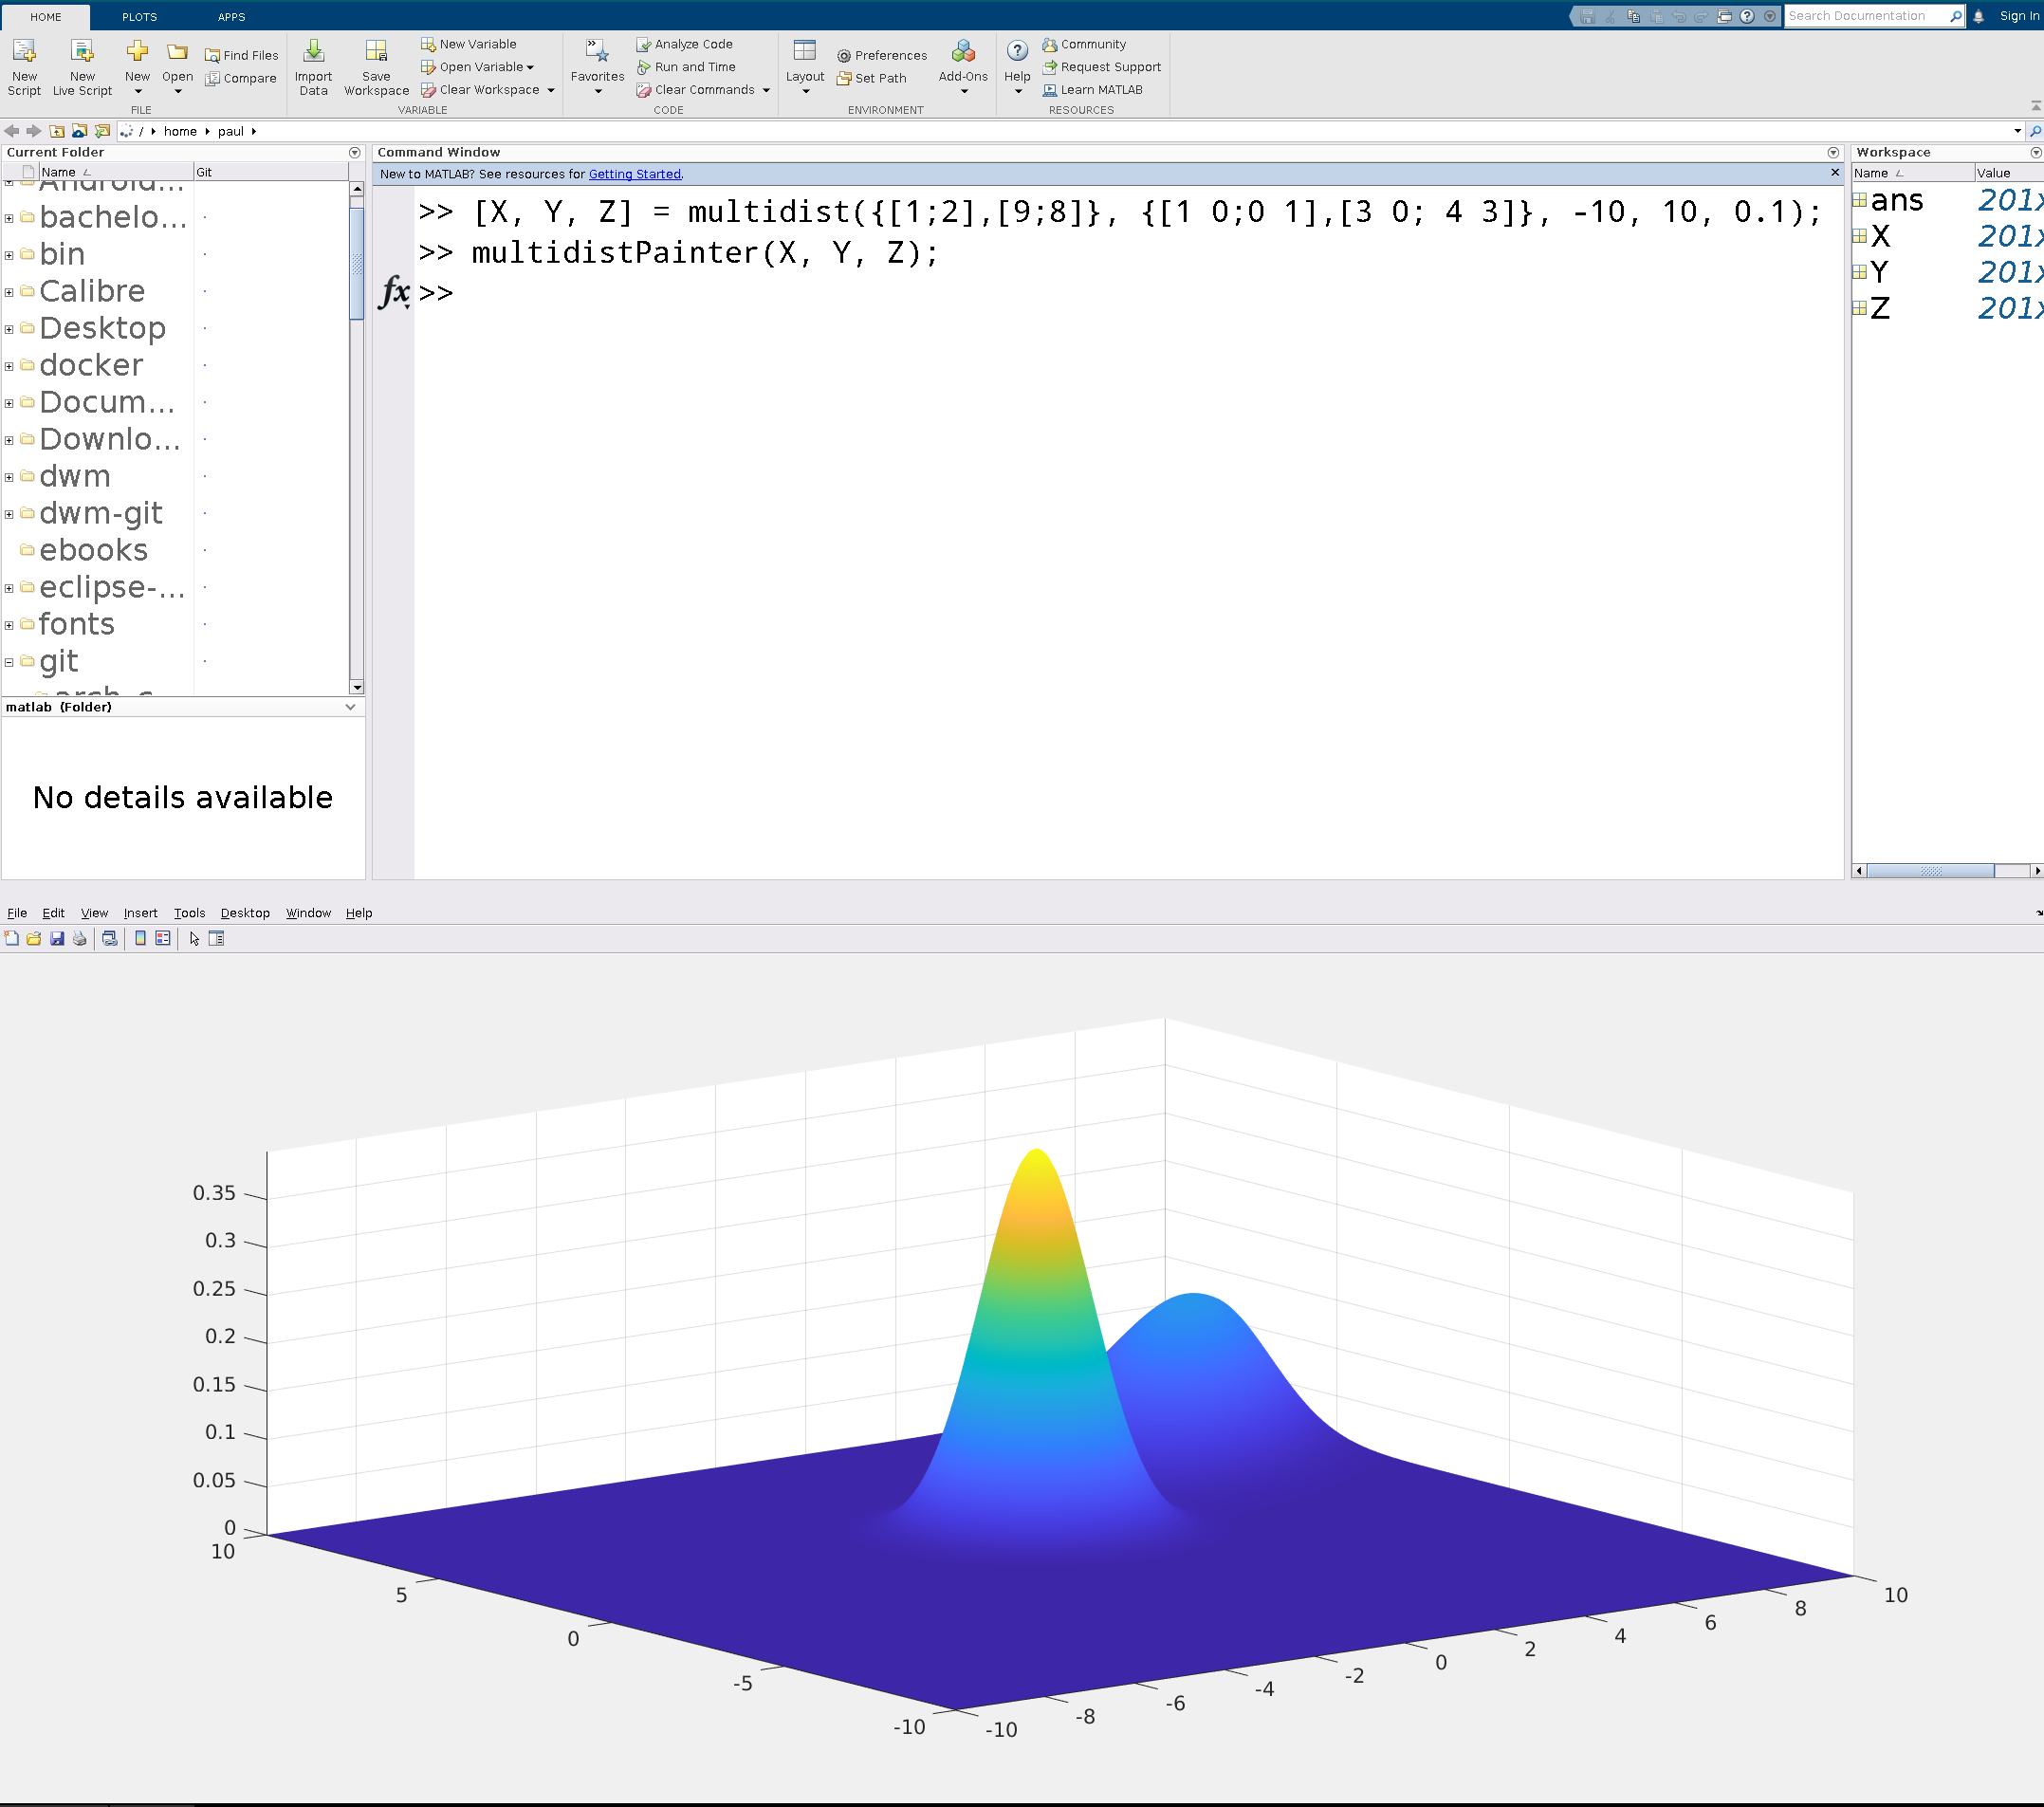
\includegraphics[scale=0.4]{./img/multidist_01.png}
		\end{figure}
		\newpage

	\item Run 2
		\begin{figure}[H]
			\centering
			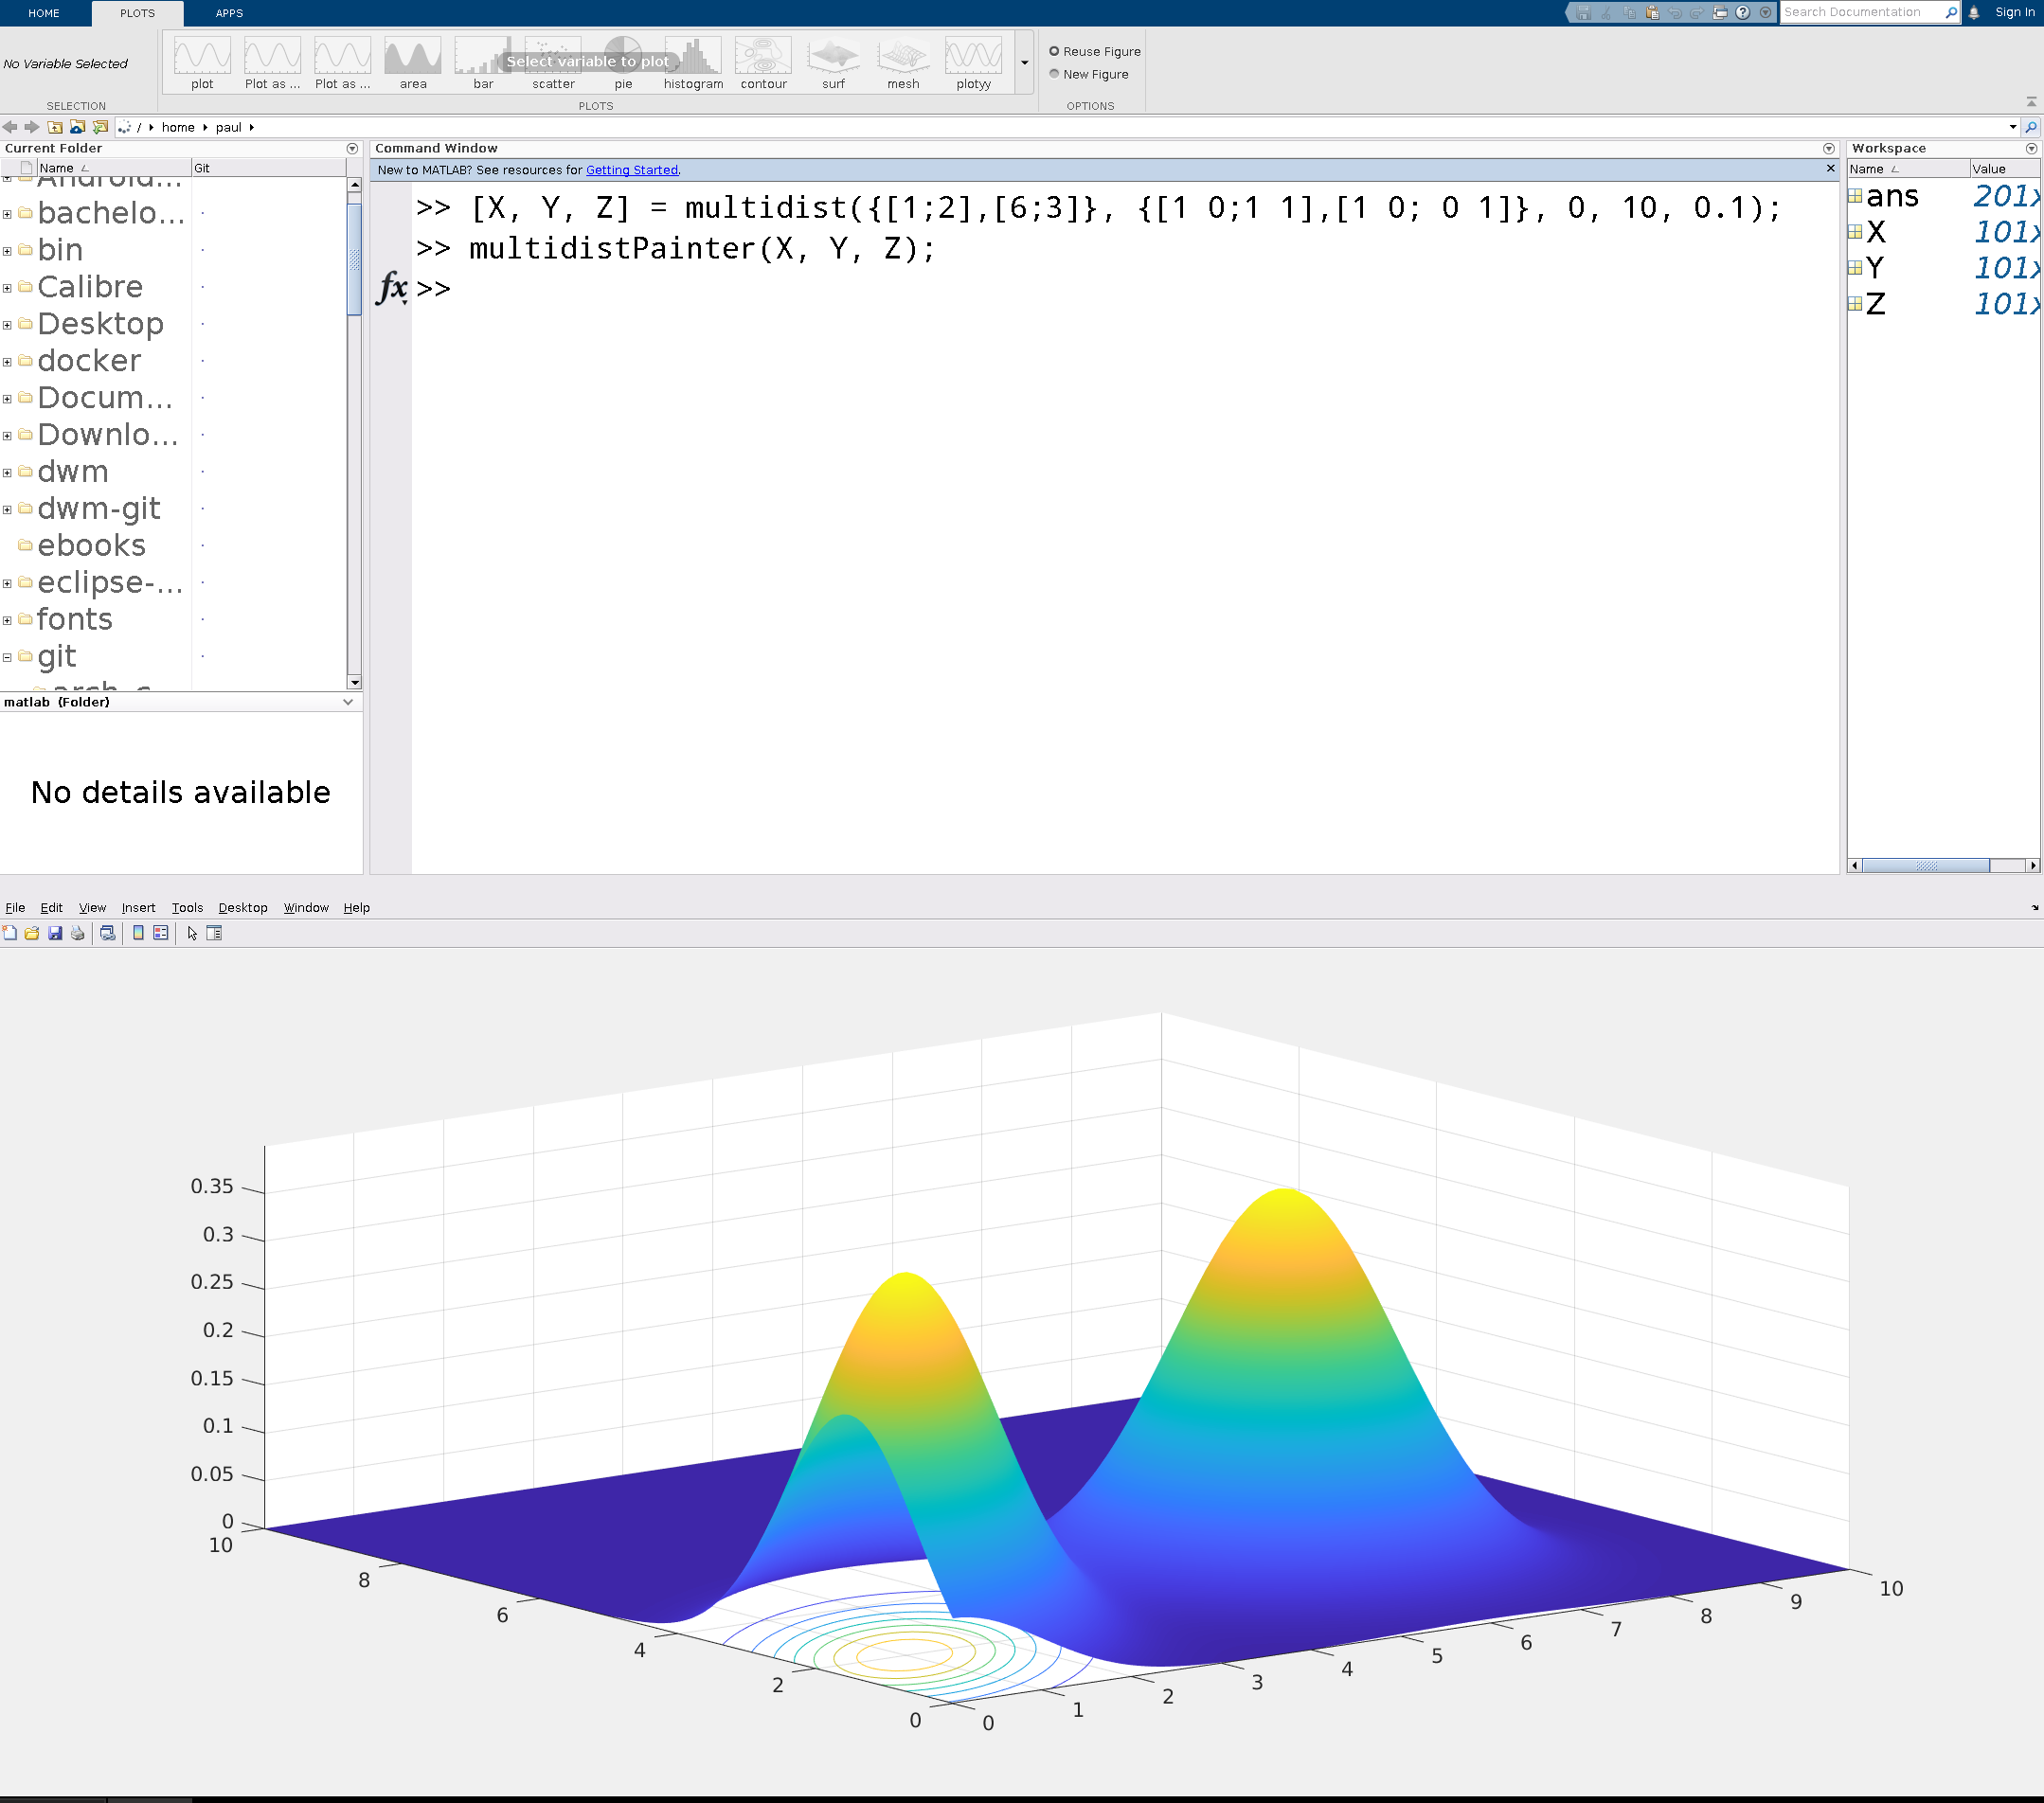
\includegraphics[scale=0.4]{./img/multidist_02.png}
		\end{figure}
\end{enumerate}
\end{document}
